\section{Resultados}

A tabela \ref{tab:eval} mostra a acurácia do modelo classificando imagens do conjunto de teste.

\begin{table}[h!]
  \centering

  \caption{Acurácia no conjunto de teste para os modelos.}
  \label{tab:eval}

  \begin{tabular}{cc}
    \toprule
    Modelo & Acurácia no conjunto de teste \\
    \midrule
    1      & 86,82\%                       \\
    2      & 88,43\%                       \\
    3      & 83,68\%                       \\
    \bottomrule
  \end{tabular}
\end{table}


Uma das formas de inspecionar o aprendizado de uma rede neural artificial é pela análise dos gráficos da acurácia e perda em cada época do treinamento, como mostrado nas figuras \ref{fig:mod1_treinamento}, \ref{fig:mod2_treinamento} e \ref{fig:mod3_treinamento}. Estes gráficos permitem ver o quanto a rede suporta ser treinada e também detectar \emph{overfiting}\footnote{Excesso de treinamento de uma rede neural articial.}.

Outra forma é pela curva ROC (\emph{Receiver Operating Characteristic}), como nas figuras \ref{fig:mod1_roc}, \ref{fig:mod2_roc} e \ref{fig:mod3_roc}. Ela é uma medição de desempenho para problemas de classificação em várias configurações de limites. ROC é uma curva de probabilidade e AUC (\emph{Area Under Curve}) representa o grau de separabilidade. Isto é, diz o quanto o modelo é capaz de distinguir entre classes. \cite{Fawcett2006,Hanley1982}

Pela análise dos gráficos da figura \ref{fig:graficos}, vemos que os modelos 1 e 2, que são treinados com menos informação -- apenas 3 bandas, tem uma maior sensibilidade, ou seja, consegue distinguir melhor entre as classes em relação ao modelo 3, treinado com 12 bandas fotométricas.

% Pela figura \ref{fig:conv_train}, é visto que o \emph{overfiting} começa na oitava época de treinamento. A partir daí, a curva de perda do conjunto de validação começa a divergir da curva de perda do conjunto de treinamento.

% Já na figura \ref{fig:pretrained_train}, é visto que o \emph{overfiting} começa na décima segunda época de treinamento. No entanto, a acurácia final desta rede é menor que da primeira, mesmo com mais épocas de treinamento.

% \pagebreak
\afterpage{\clearpage}

\begin{figure}[!t]
  \centering
  % \vspace{-20pt}
  \begin{subfigure}{.5\textwidth}
    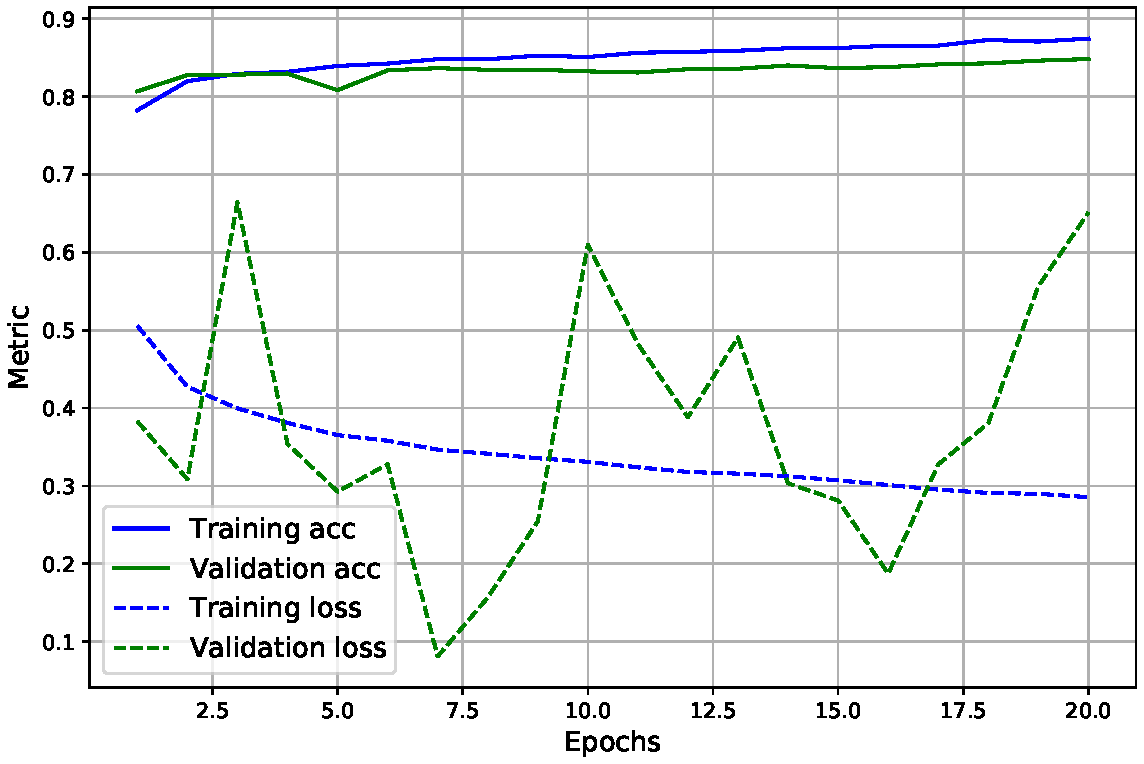
\includegraphics[width=.98\linewidth,left]{figures/sdss_conv_train.pdf}
    \caption{Modelo 1: Treinamento}
    \label{fig:mod1_treinamento}
  \end{subfigure}%
  \begin{subfigure}{.5\textwidth}
    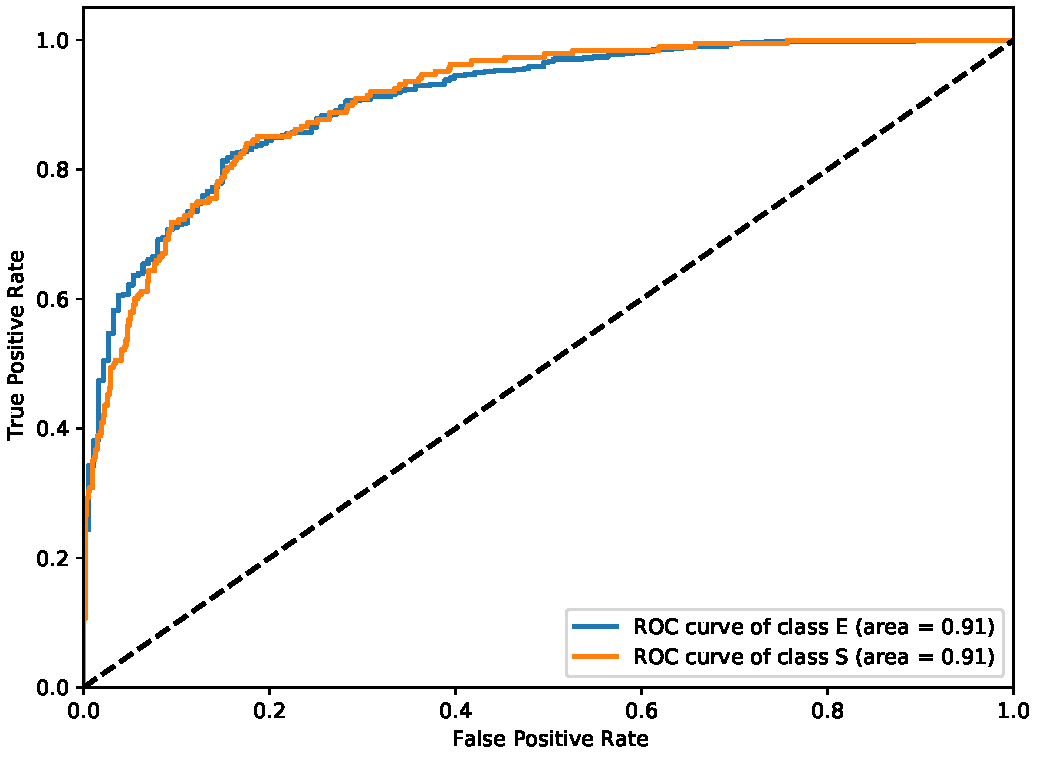
\includegraphics[width=.98\linewidth,right]{figures/roc_sdss_conv.pdf}
    \caption{Modelo 1: ROC}
    \label{fig:mod1_roc}
  \end{subfigure}\\[3mm]
  \begin{subfigure}{.5\textwidth}
    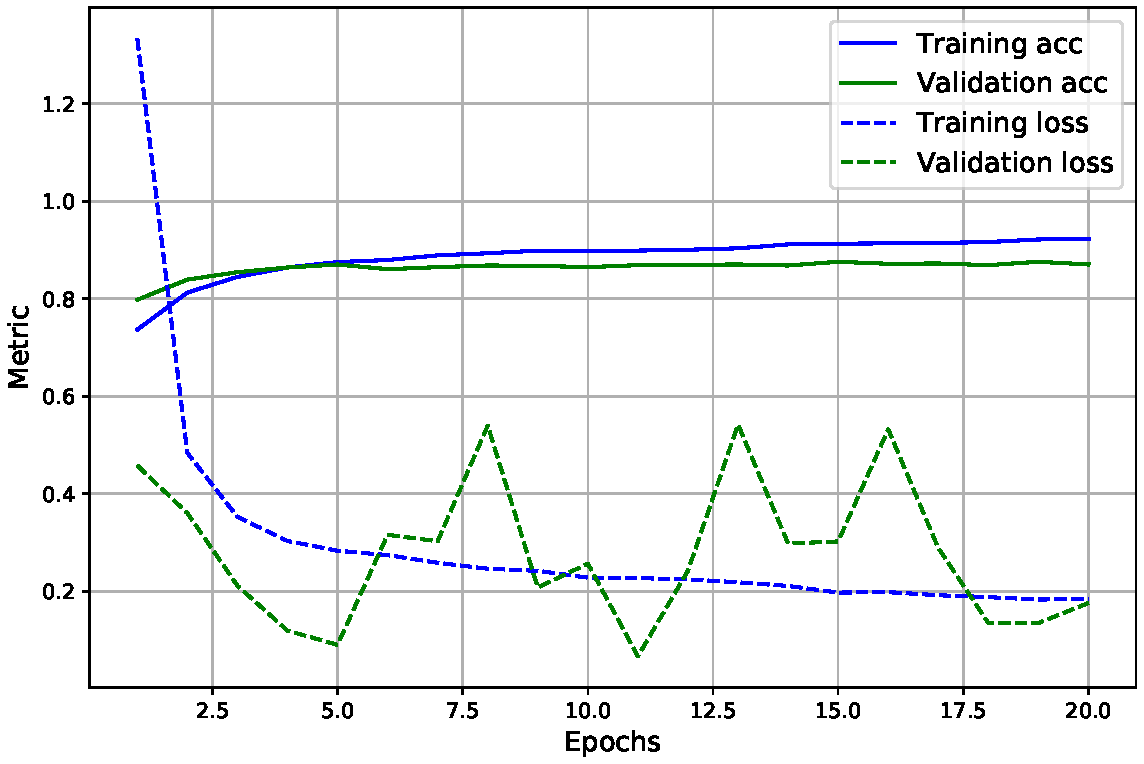
\includegraphics[width=.98\linewidth,left]{figures/sdss_pretrained_train.pdf}
    \caption{Modelo 2: Treinamento}
    \label{fig:mod2_treinamento}
  \end{subfigure}%
  \begin{subfigure}{.5\textwidth}
    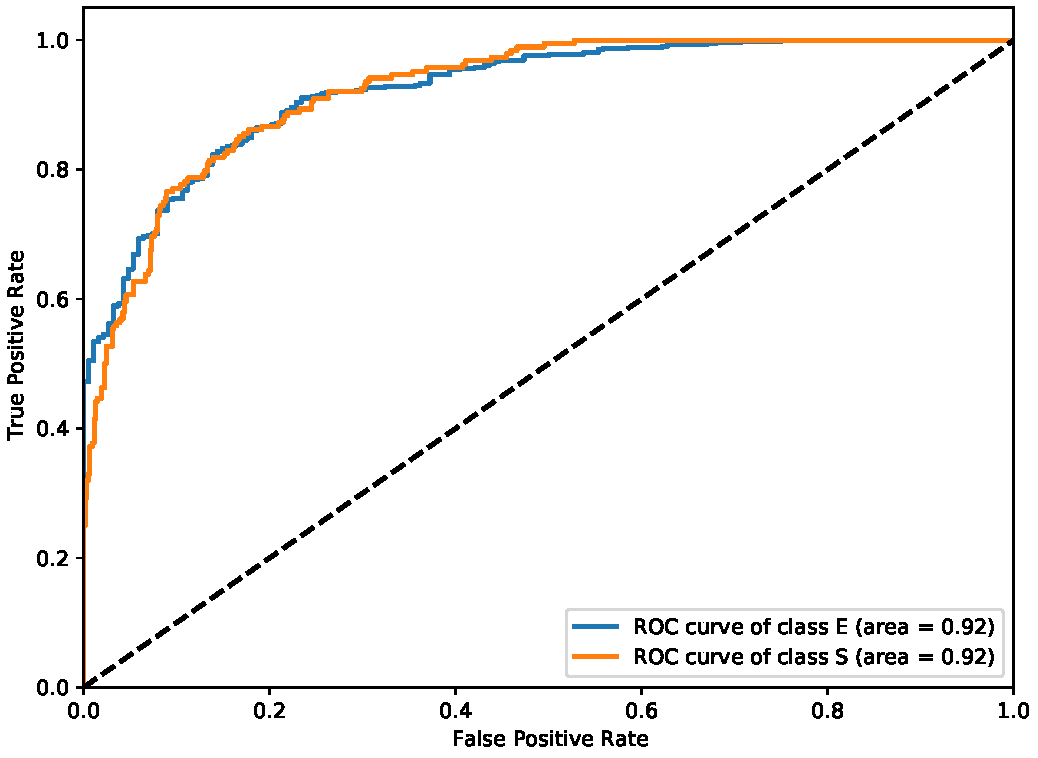
\includegraphics[width=.98\linewidth,right]{figures/roc_sdss_pretrained.pdf}
    \caption{Modelo 2: ROC}
    \label{fig:mod2_roc}
  \end{subfigure}\\[3mm]
  \begin{subfigure}{.5\textwidth}
    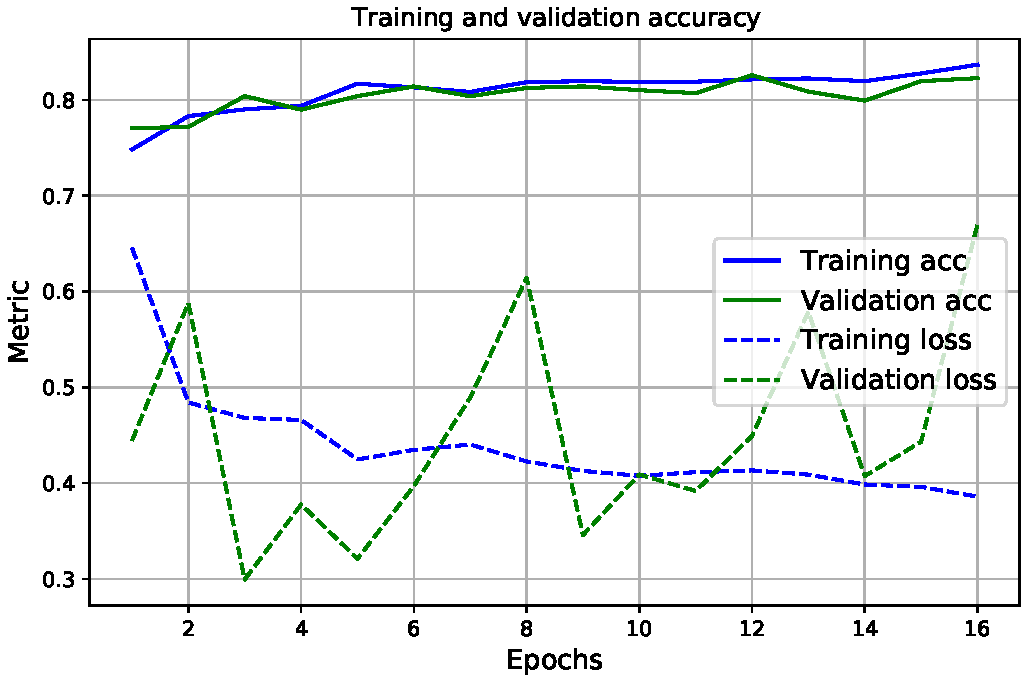
\includegraphics[width=.98\linewidth,left]{figures/splus_train.pdf}
    \caption{Modelo 3: Treinamento}
    \label{fig:mod3_treinamento}
  \end{subfigure}%
  \begin{subfigure}{.5\textwidth}
    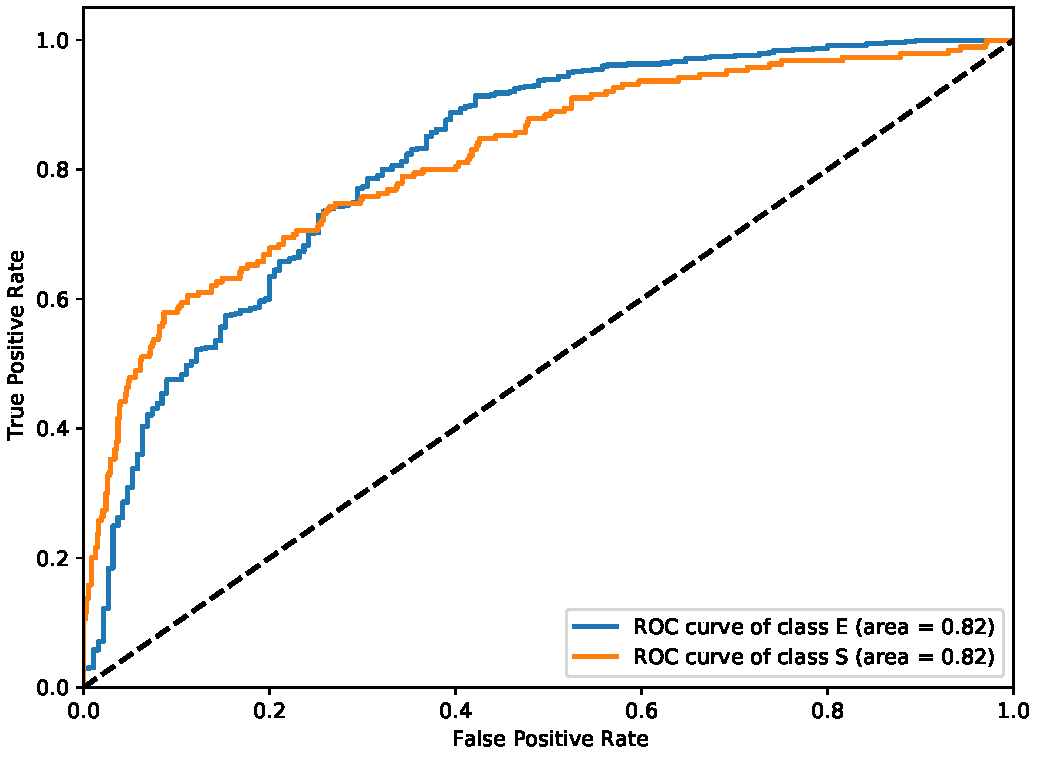
\includegraphics[width=.98\linewidth,right]{figures/roc_splus.pdf}
    \caption{Modelo 3: ROC}
    \label{fig:mod3_roc}
  \end{subfigure}
  \caption{Gráficos do treinamento e respectiva curva ROC para cada modelo.}
  \label{fig:graficos}
\end{figure}

% \begin{figure}[h!]
%   \centering
%   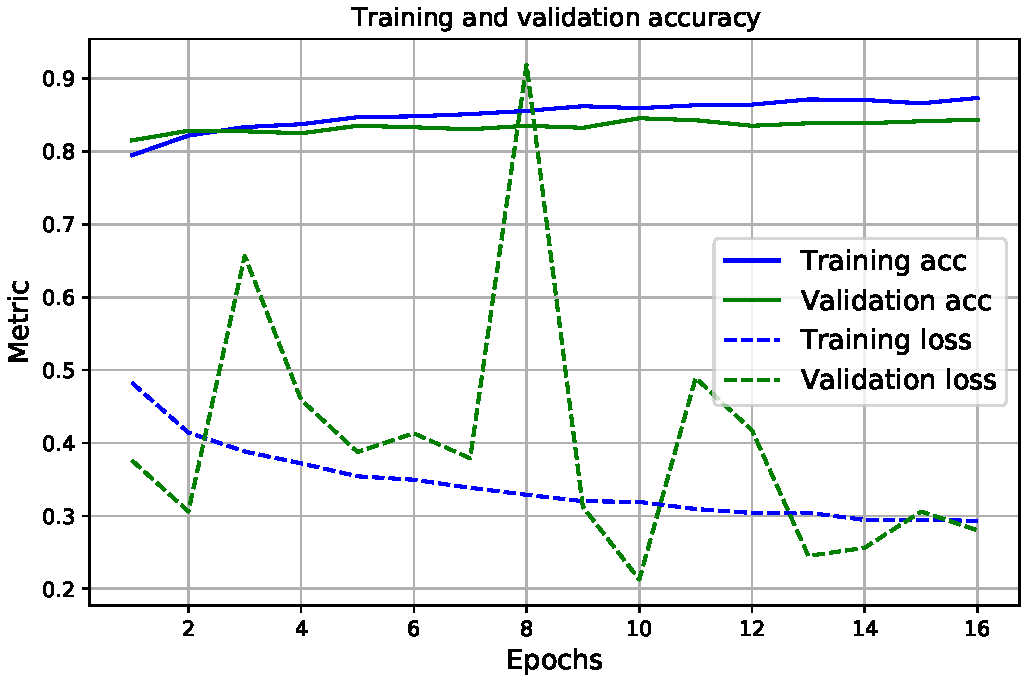
\includegraphics[width=.79\textwidth]{figures/conv_train2.pdf}
%   \caption{Gráfico da acurácia e perda dos subconjuntos de treino e validação em cada época de treinamento do Modelo 1.}
%   \label{fig:conv_train}
% \end{figure}

% \begin{figure}[h!]
%   \centering
%   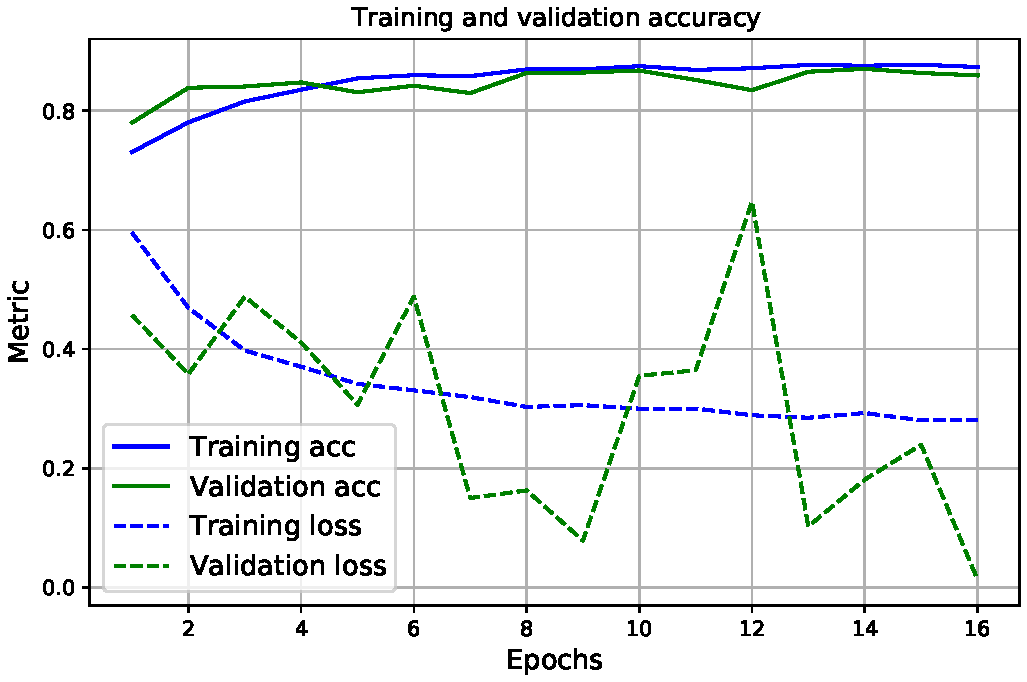
\includegraphics[width=.79\textwidth]{figures/pretrained_train2.pdf}
%   \caption{Gráfico da acurácia e perda dos subconjuntos de treino e validação em cada época de treinamento do Modelo 2.}
%   \label{fig:pretrained_train}
% \end{figure}

% \begin{figure}[h!]
%   \centering
%   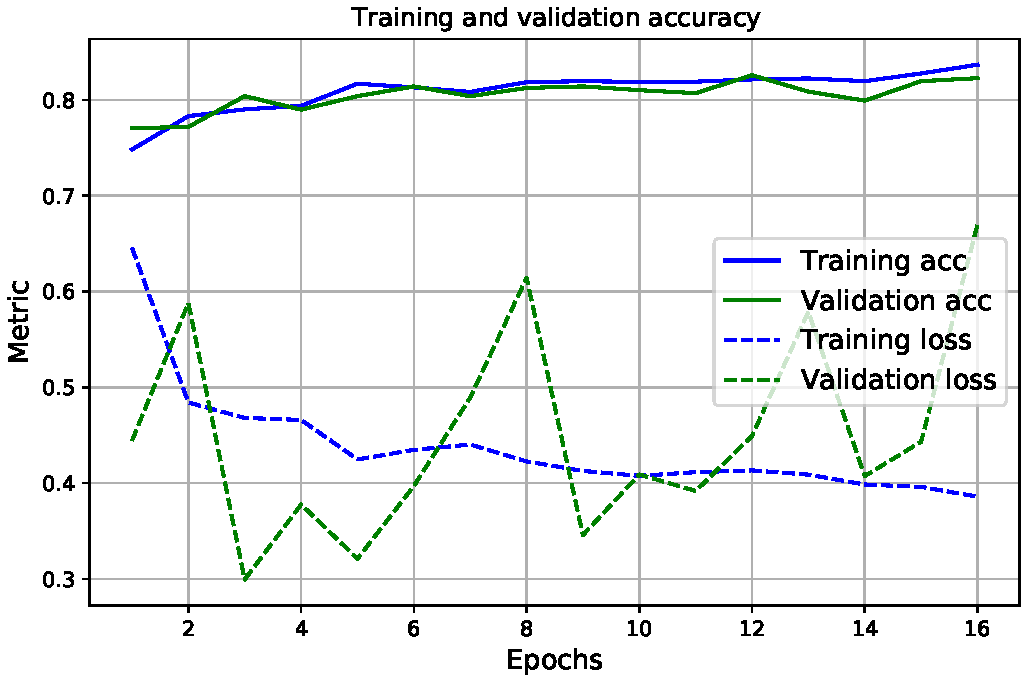
\includegraphics[width=.79\textwidth]{figures/splus_train.pdf}
%   \caption{Gráfico da acurácia e perda dos subconjuntos de treino e validação em cada época de treinamento do Modelo 3.}
%   \label{fig:splus_train}
% \end{figure}
